\documentclass[border=3pt]{standalone}
\usepackage{fontspec}
\setmainfont{DejaVu Serif}
\usepackage{pgfplots}
\pgfplotsset{compat=1.18}
\usetikzlibrary{arrows.meta,calc,positioning,shapes.geometric}
\definecolor{forest}{HTML}{346E57}
\definecolor{sage}{HTML}{E8EFEA}
\definecolor{clay}{HTML}{B77E60}
\definecolor{gray}{HTML}{718078}
\definecolor{rule}{HTML}{B7C3BA}
\definecolor{ink}{HTML}{000000}
\begin{document}
\hyphenpenalty=10000\exhyphenpenalty=10000
\fontsize{11}{13.2}\selectfont
\renewcommand{\small}{\fontsize{9.9}{12.1}\selectfont}
\renewcommand{\scriptsize}{\fontsize{8.8}{11}\selectfont}
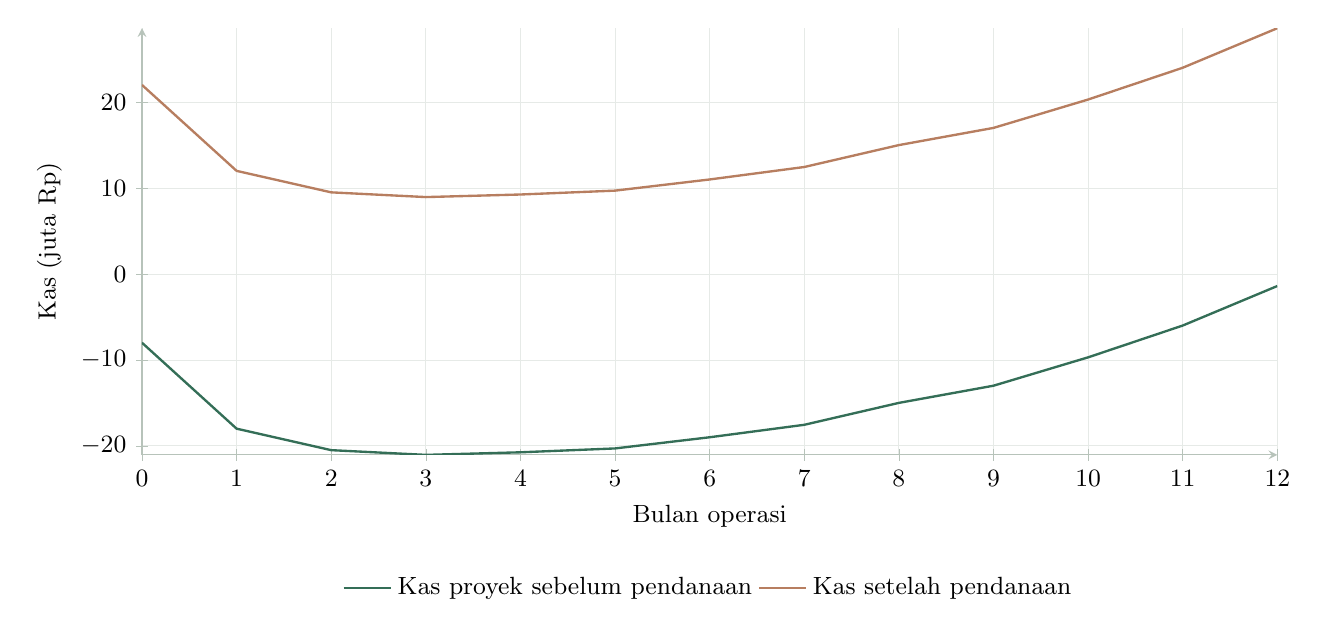
\begin{tikzpicture}\begin{axis}[width=16cm,height=7cm,scale only axis=false,
axis lines=left,axis line style={draw=rule},tick style={draw=rule},
tick label style={font=\small},label style={font=\small},
grid=major,grid style={draw=rule!35,line width=.3pt},
legend style={draw=none,fill=none,font=\small,at={(.5,-.26)},anchor=north},legend columns=-1,
xlabel={Bulan operasi},ylabel={Kas (juta Rp)},]
\addplot+[mark=none,color=forest,line width=.85pt] coordinates {(0,-8) (1,-18) (2,-20.5) (3,-21.05) (4,-20.75) (5,-20.3) (6,-19) (7,-17.55) (8,-15) (9,-13) (10,-9.7) (11,-6) (12,-1.4)};
\addlegendentry{Kas proyek sebelum pendanaan}
\addplot+[mark=none,color=clay,line width=.85pt] coordinates {(0,22) (1,12) (2,9.5) (3,8.95) (4,9.25) (5,9.7) (6,11) (7,12.45) (8,15) (9,17) (10,20.3) (11,24) (12,28.6)};
\addlegendentry{Kas setelah pendanaan}
\end{axis}\end{tikzpicture}
\end{document}
